% Per-percentile ns/op bar chart for baseline vs candidate.
% Same data as Table 1; shows the asymmetry between min (slight regression)
% and median/p25 (large improvement) more vividly than the table alone.
%
% USAGE in paper.tex:
%   \usepackage{pgfplots}
%   \pgfplotsset{compat=1.18}
%   ...
%   \begin{figure}
%     \centering
%     % Per-percentile ns/op bar chart for baseline vs candidate.
% Same data as Table 1; shows the asymmetry between min (slight regression)
% and median/p25 (large improvement) more vividly than the table alone.
%
% USAGE in paper.tex:
%   \usepackage{pgfplots}
%   \pgfplotsset{compat=1.18}
%   ...
%   \begin{figure}
%     \centering
%     % Per-percentile ns/op bar chart for baseline vs candidate.
% Same data as Table 1; shows the asymmetry between min (slight regression)
% and median/p25 (large improvement) more vividly than the table alone.
%
% USAGE in paper.tex:
%   \usepackage{pgfplots}
%   \pgfplotsset{compat=1.18}
%   ...
%   \begin{figure}
%     \centering
%     % Per-percentile ns/op bar chart for baseline vs candidate.
% Same data as Table 1; shows the asymmetry between min (slight regression)
% and median/p25 (large improvement) more vividly than the table alone.
%
% USAGE in paper.tex:
%   \usepackage{pgfplots}
%   \pgfplotsset{compat=1.18}
%   ...
%   \begin{figure}
%     \centering
%     \input{figs/bench-improvement-bars}
%     \caption{Per-percentile ns/op of \texttt{BenchmarkProposal3Nodes}
%              across 10 paired runs. Bars below their baseline counterpart
%              are improvements.}
%     \label{fig:bench-bars}
%   \end{figure}
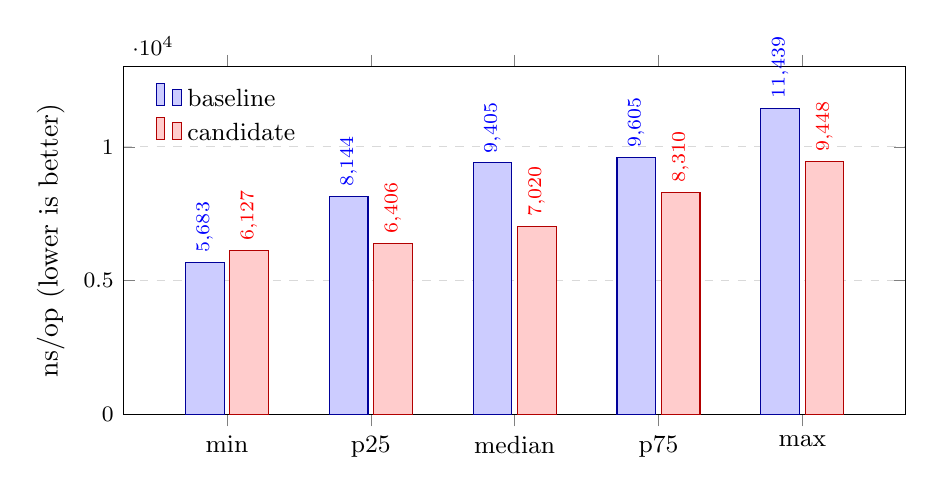
\begin{tikzpicture}
  \begin{axis}[
    width=0.95\linewidth,
    height=6cm,
    ybar=2pt,
    bar width=14pt,
    enlarge x limits=0.18,
    ylabel={ns/op (lower is better)},
    symbolic x coords={min, p25, median, p75, max},
    xtick=data,
    xticklabel style={font=\small},
    yticklabel style={font=\footnotesize},
    ymin=0, ymax=13000,
    ymajorgrids=true, grid style={dashed,gray!30},
    nodes near coords,
    nodes near coords style={font=\scriptsize, rotate=90, anchor=west},
    legend pos=north west,
    legend style={font=\small, draw=none, fill=none},
    legend cell align=left,
  ]
    \addplot+[draw=blue!60!black, fill=blue!20] coordinates {
      (min,5683) (p25,8144) (median,9405) (p75,9605) (max,11439)
    };
    \addlegendentry{baseline}
    \addplot+[draw=red!70!black, fill=red!20] coordinates {
      (min,6127) (p25,6406) (median,7020) (p75,8310) (max,9448)
    };
    \addlegendentry{candidate}
  \end{axis}
\end{tikzpicture}

%     \caption{Per-percentile ns/op of \texttt{BenchmarkProposal3Nodes}
%              across 10 paired runs. Bars below their baseline counterpart
%              are improvements.}
%     \label{fig:bench-bars}
%   \end{figure}
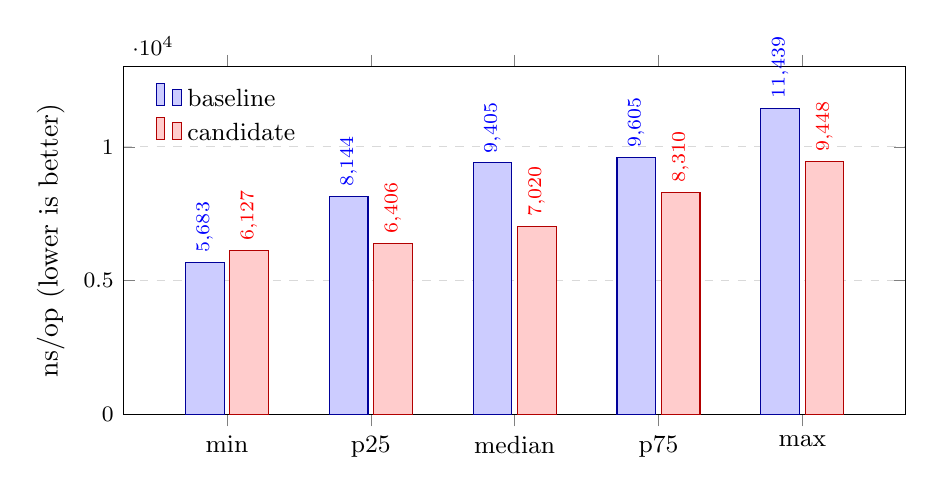
\begin{tikzpicture}
  \begin{axis}[
    width=0.95\linewidth,
    height=6cm,
    ybar=2pt,
    bar width=14pt,
    enlarge x limits=0.18,
    ylabel={ns/op (lower is better)},
    symbolic x coords={min, p25, median, p75, max},
    xtick=data,
    xticklabel style={font=\small},
    yticklabel style={font=\footnotesize},
    ymin=0, ymax=13000,
    ymajorgrids=true, grid style={dashed,gray!30},
    nodes near coords,
    nodes near coords style={font=\scriptsize, rotate=90, anchor=west},
    legend pos=north west,
    legend style={font=\small, draw=none, fill=none},
    legend cell align=left,
  ]
    \addplot+[draw=blue!60!black, fill=blue!20] coordinates {
      (min,5683) (p25,8144) (median,9405) (p75,9605) (max,11439)
    };
    \addlegendentry{baseline}
    \addplot+[draw=red!70!black, fill=red!20] coordinates {
      (min,6127) (p25,6406) (median,7020) (p75,8310) (max,9448)
    };
    \addlegendentry{candidate}
  \end{axis}
\end{tikzpicture}

%     \caption{Per-percentile ns/op of \texttt{BenchmarkProposal3Nodes}
%              across 10 paired runs. Bars below their baseline counterpart
%              are improvements.}
%     \label{fig:bench-bars}
%   \end{figure}
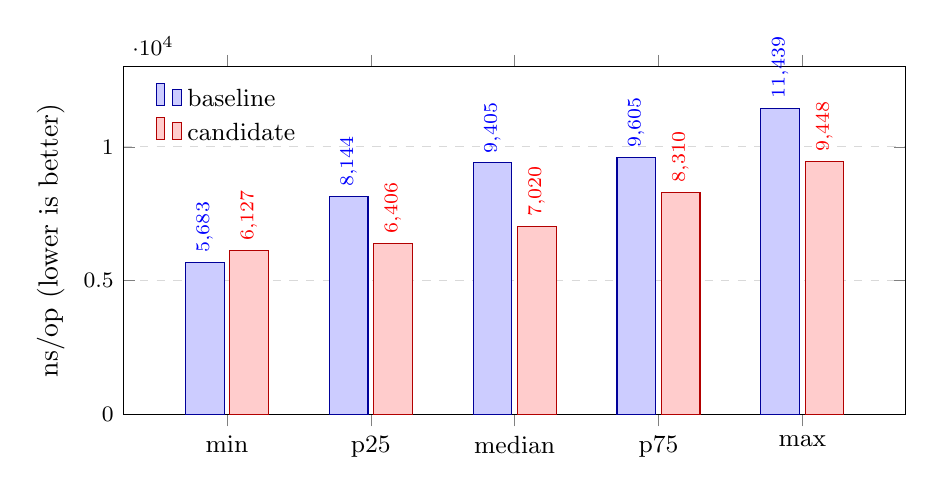
\begin{tikzpicture}
  \begin{axis}[
    width=0.95\linewidth,
    height=6cm,
    ybar=2pt,
    bar width=14pt,
    enlarge x limits=0.18,
    ylabel={ns/op (lower is better)},
    symbolic x coords={min, p25, median, p75, max},
    xtick=data,
    xticklabel style={font=\small},
    yticklabel style={font=\footnotesize},
    ymin=0, ymax=13000,
    ymajorgrids=true, grid style={dashed,gray!30},
    nodes near coords,
    nodes near coords style={font=\scriptsize, rotate=90, anchor=west},
    legend pos=north west,
    legend style={font=\small, draw=none, fill=none},
    legend cell align=left,
  ]
    \addplot+[draw=blue!60!black, fill=blue!20] coordinates {
      (min,5683) (p25,8144) (median,9405) (p75,9605) (max,11439)
    };
    \addlegendentry{baseline}
    \addplot+[draw=red!70!black, fill=red!20] coordinates {
      (min,6127) (p25,6406) (median,7020) (p75,8310) (max,9448)
    };
    \addlegendentry{candidate}
  \end{axis}
\end{tikzpicture}

%     \caption{Per-percentile ns/op of \texttt{BenchmarkProposal3Nodes}
%              across 10 paired runs. Bars below their baseline counterpart
%              are improvements.}
%     \label{fig:bench-bars}
%   \end{figure}
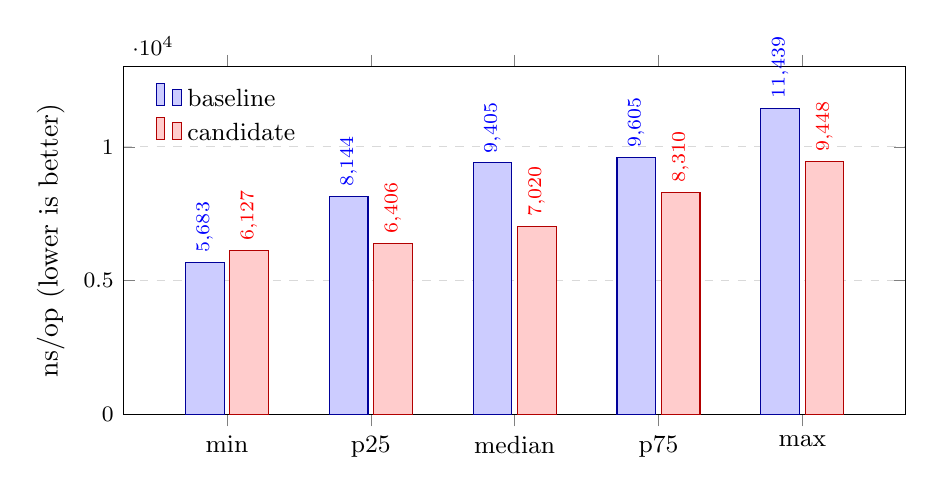
\begin{tikzpicture}
  \begin{axis}[
    width=0.95\linewidth,
    height=6cm,
    ybar=2pt,
    bar width=14pt,
    enlarge x limits=0.18,
    ylabel={ns/op (lower is better)},
    symbolic x coords={min, p25, median, p75, max},
    xtick=data,
    xticklabel style={font=\small},
    yticklabel style={font=\footnotesize},
    ymin=0, ymax=13000,
    ymajorgrids=true, grid style={dashed,gray!30},
    nodes near coords,
    nodes near coords style={font=\scriptsize, rotate=90, anchor=west},
    legend pos=north west,
    legend style={font=\small, draw=none, fill=none},
    legend cell align=left,
  ]
    \addplot+[draw=blue!60!black, fill=blue!20] coordinates {
      (min,5683) (p25,8144) (median,9405) (p75,9605) (max,11439)
    };
    \addlegendentry{baseline}
    \addplot+[draw=red!70!black, fill=red!20] coordinates {
      (min,6127) (p25,6406) (median,7020) (p75,8310) (max,9448)
    };
    \addlegendentry{candidate}
  \end{axis}
\end{tikzpicture}
